\pdfinfoomitdate=1
\pdftrailerid{}
\documentclass[tikz,border=4pt]{standalone}
\usepackage{newtxtext}
\usetikzlibrary{arrows.meta,positioning,shapes.geometric}
\definecolor{blue}{HTML}{0072B2}
\definecolor{orange}{HTML}{E69F00}
\definecolor{green}{HTML}{009E73}
\definecolor{purple}{HTML}{7B61A8}
\definecolor{graybox}{HTML}{E8E8E8}
\tikzset{
  stage/.style={draw=black,rounded corners=2pt,very thick,minimum width=37mm,
    minimum height=24mm,align=center,font=\sffamily\small,fill=white},
  active/.style={stage,fill=blue!9,draw=blue},
  correction/.style={stage,fill=orange!12,draw=orange},
  open/.style={stage,fill=graybox,draw=black,dashed},
  flow/.style={-{Latex[length=3mm]},very thick,draw=black}
}
\begin{document}
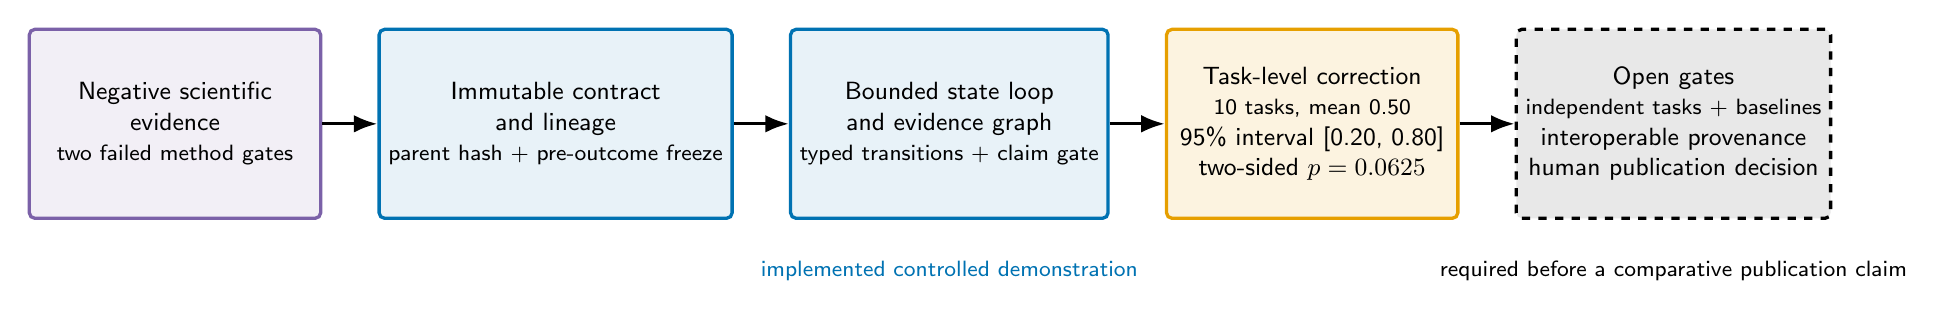
\begin{tikzpicture}[node distance=7mm]
  \node[stage,fill=purple!10,draw=purple] (negative) {Negative scientific\\evidence\\\footnotesize two failed method gates};
  \node[active,right=of negative] (freeze) {Immutable contract\\and lineage\\\footnotesize parent hash + pre-outcome freeze};
  \node[active,right=of freeze] (loop) {Bounded state loop\\and evidence graph\\\footnotesize typed transitions + claim gate};
  \node[correction,right=of loop] (analysis) {Task-level correction\\\footnotesize 10 tasks, mean 0.50\\95\% interval [0.20, 0.80]\\two-sided $p=0.0625$};
  \node[open,right=of analysis] (external) {Open gates\\\footnotesize independent tasks + baselines\\interoperable provenance\\human publication decision};
  \draw[flow] (negative) -- (freeze);
  \draw[flow] (freeze) -- (loop);
  \draw[flow] (loop) -- (analysis);
  \draw[flow] (analysis) -- (external);
  \node[font=\sffamily\footnotesize,text=blue,below=4mm of loop] {implemented controlled demonstration};
  \node[font=\sffamily\footnotesize,text=black,below=4mm of external] {required before a comparative publication claim};
\end{tikzpicture}
\end{document}
